\documentclass[12pt]{article}

\usepackage{booktabs}
\usepackage{tikz}
\usepackage{pgfplots}
\pgfplotsset{compat=1.18}
\usepackage{worldflags}

\usepackage[a4paper, width = 160mm, top = 35mm, bottom = 30mm, 
bindingoffset = 0mm]{geometry}
\usepackage[utf8]{inputenc}
\usepackage[T1]{fontenc}
\usepackage{fancyhdr}
\usepackage{hyperref}
\hypersetup{
  colorlinks = true,
  linkcolor = black,
  urlcolor = black,
  citecolor = black}
\pagestyle{fancy}
\fancyhead{}
\fancyhead[R]{\changefont{\mytitle}}
\fancyfoot{}
\fancyfoot[R]{\thepage}
\setlength{\headheight}{14.5pt}
\setlength{\parindent}{0pt}
\interfootnotelinepenalty = 10000

% MAIN -----------------------------------

\newcommand{\mytitle}{Formuła 1 - Podsumowanie sezonu 2022}
\newcommand{\myname}{Radosław Terelak}
\newcommand{\changefont}{%
    \fontsize{8}{11}\selectfont
}

\renewcommand*\contentsname{Spis treści}
\renewcommand{\abstractname}{Streszczenie}
\renewcommand{\figurename}{Obraz}
\renewcommand{\tablename}{Tabela}
\begin{document}

% FRONT PAGE ------------------------------------------
 
\begin{titlepage}
\begin{center}
    
\LARGE
LaTeX dla Informatyków
    
\vspace{0.5cm}
      
\rule{\textwidth}{1.5pt}
\LARGE
\textbf{\mytitle}
\rule{\textwidth}{1.5pt}
   
\vspace{0.5cm}
      
\large
Politechnika Śląska\\
Wydział Matematyki Stosowanej

\vfill

\Large
\textbf{\myname}

\vfill

\large
Gliwice, 2023
      
\vfill


\includegraphics[width = 0.5\textwidth]{img/logoMS}

\vfill

\end{center}
\end{titlepage}

% CONTENTS -------------------------------

\newpage
\tableofcontents
\begin{abstract}
    Niniejszy artykuł podsumowuje wydarzenia z wyścigów Formuły 1 sezonu 2022. Znajdują się tu tabele z klasyfikacjami mistrzostw, kalendarzem wszystkich odbytych wyścigów jak i najważniejsze informacje oraz subiektywne zdanie na temat wygranych i przegranych rywalizacji w tym roku. 
\end{abstract}

% CHAPTERS -------------------------------
    
\newpage
\section{Wstęp}
Mistrzostwa Świata Formuły 1 FIA 2022 były 73. edycją Mistrzostw Świata Formuły 1. Są uznawane przez Fédération Internationale de l'Automobile (FIA), jako najwyższej klasy rywalizacja samochodów wyścigowych. Mistrzostwa były rozgrywane w ramach dwudziestu dwóch Grand Prix, które odbywały się na całym świecie i zakończyły się wcześniej niż w innych ostatnich latach, aby uniknąć nakładania się z Mistrzostwami Świata FIFA w Katarze.\\

Kierowcy i zespoły rywalizowały odpowiednio o tytuły Mistrza Świata Kierowców i Mistrza Świata Konstruktorów. W tym roku wprowadzono istotne zmiany w przepisach technicznych tego sportu. Zmiany te miały zostać wprowadzone w 2021 roku, ale zostały przesunięte do 2022 r. ze względu na pandemię COVID-19.\\ 

Max Verstappen, który był aktualnym mistrzem kierowców, zdobył swój drugi tytuł podczas Grand Prix Japonii, podczas gdy jego zespół, Red Bull Racing, zdobył swoje piąte mistrzostwo świata konstruktorów i pierwsze od 2013 roku podczas kolejnego Grand Prix Stanów Zjednoczonych. Mercedes był panującym mistrzem konstruktorów.\\

To był ostatni sezon czterokrotnego mistrza świata Sebastiana Vettela. Siedmiokrotny mistrz świata Lewis Hamilton przeżył trudny sezon z Mercedesem, nie zdobywając ani pole position, ani zwycięstwa w Grand Prix w trakcie sezonu, co zdarzyło się po raz pierwszy w jego karierze w Formule 1 od jej początku w 2007 roku.

\begin{figure}[ht]
    \centering
    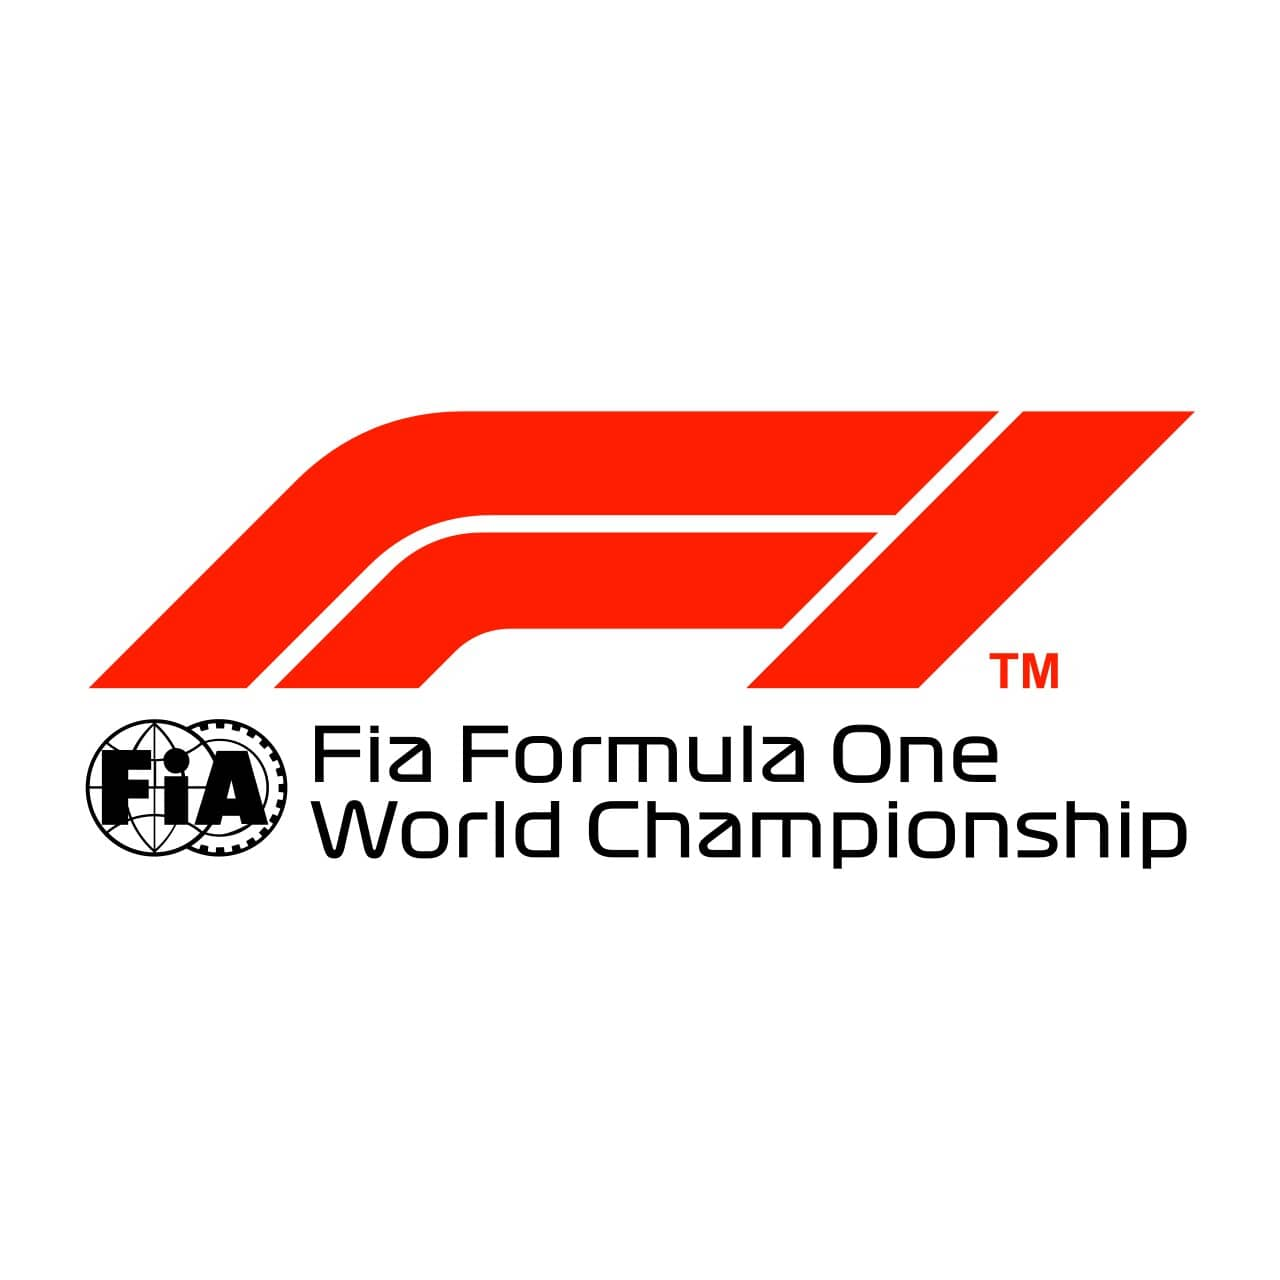
\includegraphics[scale = 0.2]{img/f1-logo}
    \caption{Logo Mistrzostw Świata Formuły 1 FIA}
    \label{fig:logo-f1}
\end{figure}

\newpage
\section{Kalendarz}

W kalendarzu znalazł się nowy wyścig - Grand Prix Miami. Areną zmagań został tor Miami International Autodrome, zlokalizowany wokół Hard Rock Stadium. Dzięki temu, po raz pierwszy od 1984 odbyły się dwa wyścigi Formuły 1 w Stanach Zjednoczonych w jednym sezonie.\\
Grand Prix Australii, Grand Prix Kanady, Grand Prix Singapuru oraz Grand Prix Japonii powróciły po dwóch latach przerwy. W sezonach 2020 i 2021 wyścigi były odwołane wskutek pandemii COVID-19.\\
Z kalendarza zniknęły wyścigi o Grand Prix Portugalii, Grand Prix Styrii oraz Grand Prix Turcji. Grand Prix Rosji, które miało się odbyć w dniach 23–25 września, zostało odwołane wskutek inwazji Rosji na Ukrainę.

\begin{table}[ht]
    \caption{Wszystkie Grand Prix sezonu 2022}
    \centering
    \resizebox{\textwidth}{!}{%
        \begin{tabular}{@{}clll@{}}
        \toprule
        \textbf{Nr.} & \textbf{Grand Prix}                                      & \textbf{Tor}                               & \textbf{Data wyścigu} \\ \midrule
        1            & \worldflag[length=8mm, width=4mm]{BH}Bahrajnu            & Bahrain International Circuit, Sakhir      & 20 marca              \\
        2            & \worldflag[length=8mm, width=4mm]{SA}Arabii Saudyjskiej  & Jeddah Corniche Circuit, Jeddah            & 27 marca              \\
        3            & \worldflag[length=8mm, width=4mm]{AU}Australii           & Albert Park Circuit, Melbourne             & 10 kwietnia           \\
        4            & \worldflag[length=8mm, width=4mm]{IT}Emilii-Romanii      & Imola Circuit, Imola                       & 24 kwietnia           \\
        5            & \worldflag[length=8mm, width=4mm]{US}Miami               & Miami International Autodrome, Florida     & 8 maja                \\
        6            & \worldflag[length=8mm, width=4mm]{ES}Hiszpanii           & Circuit de Barcelona-Catalunya, Montmeló   & 22 maja               \\
        7            & \worldflag[length=8mm, width=4mm]{ID}Monako              & Circuit de Monaco, Monaco                  & 29 maja               \\
        8            & \worldflag[length=8mm, width=4mm]{AZ}Azerbejdżanu        & Baku City Circuit, Baku                    & 12 czerwca            \\
        9            & \worldflag[length=8mm, width=4mm]{CA}Kanady              & Circuit Gilles Villeneuve, Montréal        & 19 czerwca            \\
        10           & \worldflag[length=8mm, width=4mm]{GB}Wielkiej Brytanii   & Silverstone Circuit, Silverstone           & 3 lipca               \\
        11           & \worldflag[length=8mm, width=4mm]{AT}Austrii             & Red Bull Ring, Spielberg                   & 10 lipca              \\
        12           & \worldflag[length=8mm, width=4mm]{FR}Francji             & Circuit Paul Ricard, Le Castellet          & 24 lipca              \\
        13           & \worldflag[length=8mm, width=4mm]{HU}Węgier              & Hungaroring, Mogyoród                      & 31 lipca              \\
        14           & \worldflag[length=8mm, width=4mm]{BE}Belgii              & Circuit de Spa-Francorchamps, Stavelot     & 28 sierpnia           \\
        15           & \worldflag[length=8mm, width=4mm]{NL}Holandii            & Circuit Zandvoort, Zandvoort               & 4 września            \\
        16           & \worldflag[length=8mm, width=4mm]{IT}Włoch               & Monza Circuit, Monza                       & 11 września           \\
        17           & \worldflag[length=8mm, width=4mm]{SG}Singapuru           & Marina Bay Street Circuit, Singapore       & 2 października        \\
        18           & \worldflag[length=8mm, width=4mm]{JP}Japonii             & Suzuka International Racing Course, Suzuka & 9 paźniernika         \\
        19           & \worldflag[length=8mm, width=4mm]{US}USA                 & Circuit of the Americas, Austin, Texas     & 23 października       \\
        20           & \worldflag[length=8mm, width=4mm]{MX}Meksyku             & Autódromo Hermanos Rodríguez, Mexico City  & 30 października       \\
        21           & \worldflag[length=8mm, width=4mm]{BR}São Paulo           & Interlagos Circuit, São Paulo              & 13 listopada          \\
        22           & \worldflag[length=8mm, width=4mm]{AE}Abu Zabi            & Yas Marina Circuit, Abu Dhabi              & 20 listopada          \\ \bottomrule
        \end{tabular}}
    \label{Tab:kalendarz}
\end{table}

\newpage
\section{Klasyfikacja kierowców}
Jeśli chodzi o kierowców, to sezon został zdominowany przez Maxa Verstappena. Holender wygrał aż 15 z 22 wyścigów, komfortowo zgarniając tytuł mistrza. Na początku roku Charles Leclerc miał bolid, który pozwalał mu walczyć o zwycięstwa jednak w dalszej części sezonu popełniał błędy, strategie zespołu były równie wątpliwe oraz bolid Ferrari coraz mocniej odstawał od Red Bulla. Swoje pierwsze zwycięstwo w karierze odniósł Carlos Sainz Jr. oraz George Russell.\\

Natomiast Lewis Hamilton zaliczył szokujący rok. Nie zdobył żadnego Pole Position ani nigdzie nie zwyciężył. Na dodatek został pokonany przez nowego kolegę z zespołu, który bardzo szybko zadomowił się w stajni Mercedesa. Fernando Alonso miał najwięcej pecha jeśli chodzi o niezawodność samochodu i nie ujrzał mety aż 6 razy. 

\begin{table}[ht]
    \caption{Zestawienie zwycięstw, podiów i punktów kierowców w 2022}
    \centering
    \resizebox{\textwidth}{!}{%
    \begin{tabular}{@{}cllccc@{}}
        \toprule
        \textbf{Pozycja} & \textbf{Kierowca}                                        & \textbf{Zespół} & \textbf{Zwycięstwa} & \textbf{Podia} & \textbf{Punkty} \\ \midrule
        1                &\worldflag[length=8mm, width=4mm]{NL}Max Verstappen       & Red Bull        & 15                  & 17             & 454             \\
        2                &\worldflag[length=8mm, width=4mm]{ID}Charles Leclerc      & Ferrari         & 3                   & 11             & 308             \\
        3                &\worldflag[length=8mm, width=4mm]{MX}Sergio Pérez         & Red Bull        & 2                   & 11             & 305             \\
        4                &\worldflag[length=8mm, width=4mm]{GB}George Russell       & Mercedes        & 1                   & 8              & 275             \\
        5                &\worldflag[length=8mm, width=4mm]{ES}Carlos Sainz Jr.     & Ferrari         & 1                   & 9              & 246             \\
        6                &\worldflag[length=8mm, width=4mm]{GB}Lewis Hamilton       & Mercedes        & 0                   & 9              & 240             \\
        7                &\worldflag[length=8mm, width=4mm]{GB}Lando Norris         & McLaren         & 0                   & 1              & 122             \\
        8                &\worldflag[length=8mm, width=4mm]{FR}Esteban Ocon         & Alpine          & 0                   & 0              & 92              \\
        9                &\worldflag[length=8mm, width=4mm]{ES}Fernando Alonso      & Alpine          & 0                   & 0              & 81              \\
        10               &\worldflag[length=8mm, width=4mm]{FI}Valtteri Bottas      & Alfa Romeo      & 0                   & 0              & 49              \\
        11               &\worldflag[length=8mm, width=4mm]{AU}Daniel Ricciardo     & McLaren         & 0                   & 0              & 37              \\
        12               &\worldflag[length=8mm, width=4mm]{DE}Sebastian Vettel     & Aston Martin    & 0                   & 0              & 37              \\
        13               &\worldflag[length=8mm, width=4mm]{DK}Kevin Magnussen      & Haas            & 0                   & 0              & 25              \\
        14               &\worldflag[length=8mm, width=4mm]{FR}Pierre Gasly         & AlphaTauri      & 0                   & 0              & 23              \\
        15               &\worldflag[length=8mm, width=4mm]{CA}Lance Stroll         & Aston Martin    & 0                   & 0              & 18              \\
        16               &\worldflag[length=8mm, width=4mm]{DE}Mick Schumacher      & Haas            & 0                   & 0              & 12              \\
        17               &\worldflag[length=8mm, width=4mm]{JP}Yūki Tsunoda         & AlphaTauri      & 0                   & 0              & 12              \\
        18               &\worldflag[length=8mm, width=4mm]{CN}Zhou Guanyu          & Alfa Romeo      & 0                   & 0              & 6               \\
        19               &\worldflag[length=8mm, width=4mm]{TH}Alexander Albon      & Williams        & 0                   & 0              & 4               \\
        20               &\worldflag[length=8mm, width=4mm]{CA}Nicholas Latifi      & Williams        & 0                   & 0              & 2               \\
        21               &\worldflag[length=8mm, width=4mm]{NL}Nyck de Vries        & Williams        & 0                   & 0              & 2               \\
        22               &\worldflag[length=8mm, width=4mm]{DE}Nico Hülkenberg      & Aston Martin    & 0                   & 0              & 0               \\ \bottomrule
    \end{tabular}}
    \label{Tab:mś_kierowcy}
\end{table}

\newpage
\section{Klasyfikacja konstruktorów}
Mistrzem konstruktorów został Red Bull po raz pierwszy od 2013 roku. Przełamał passę Mercedesa, który od 2014 roku nigdy nie stracił tego tytułu. Na początku roku najszybszym bolidem dysponowało Ferrari, które najlepiej wykorzystało nowe regulacje techniczne. Jednak na przestrzeni długiego sezonu zostali pokonani pod względem rozwoju i już od połowy roku to Red Bull był najszybszym autem na torze. Mercedes w pierwszych wyścigach ledwie łapał się do pierwszej dziesiątki, jednak konsekwentne poprawki sprawiły, że na koniec roku byli tuż za Red Bullem.\\

Środek stawki był całkiem wyrównany, Mclaren oraz Alpine szli łeb w łeb jednak to zespół z Enstone był czwarty w klasyfikacji. Haas miał wyśmienity start sezonu, jednak podobnie jak i Ferrari zostali wyprzedzeni w rozwoju technicznym i pod koniec sezonu ich forma była przeciętna. Z kolei Aston Martin zaczął rok szokująco nisko, a skończył na poziomie Alpine. Jest to bardzo dobry prognostyk na rok 2023. Szczególnie zadowolony z tego faktu musi być Fernando Alonso, który dołącza do tej ekipy.\\


\begin{table}[ht]
    \caption{Zestawienie zwycięstw i punktów konstruktorów w 2022}
    \centering
    \resizebox{\textwidth}{!}{%
    \begin{tabular}{@{}clcc@{}}
        \toprule
        \textbf{Pozycja}       & \textbf{Kierowca}                                      & \textbf{Zwycięstwa} & \textbf{Punkty} \\ \midrule
        1                      & \worldflag[length=8mm, width=4mm]{AT}Red Bull          & 17                  & 759             \\
        2                      & \worldflag[length=8mm, width=4mm]{IT}Ferrari           & 4                   & 554             \\
        3                      & \worldflag[length=8mm, width=4mm]{DE}Mercedes          & 1                   & 515             \\
        4                      & \worldflag[length=8mm, width=4mm]{FR}Alpine            & 0                   & 173             \\
        5                      & \worldflag[length=8mm, width=4mm]{GB}McLaren           & 0                   & 159             \\
        6                      & \worldflag[length=8mm, width=4mm]{CH}Alfa Romeo        & 0                   & 55              \\
        7                      & \worldflag[length=8mm, width=4mm]{GB}Aston Martin      & 0                   & 55              \\
        8                      & \worldflag[length=8mm, width=4mm]{US}Haas              & 0                   & 37              \\
        9                      & \worldflag[length=8mm, width=4mm]{IT}AlphaTauri        & 0                   & 35              \\
        10                     & \worldflag[length=8mm, width=4mm]{GB}Williams          & 0                   & 8               \\ \bottomrule
    \end{tabular}}
    \label{Tab:mś_zespoły}
\end{table}

\newpage
\section{Wygrani i przegrani sezonu}
    \subsection{Najlepszy kierowca}
        \begin{center}
            \Huge \textbf{Max Verstappen}
        \end{center}
        Wybór jest oczywisty. Był to rekordy sezon w wykonaniu holenderskiego kierowcy. 15 zwycięstw Verstappena - nowy rekord Formuły 1 - to coś, co zapamiętamy na długo. Wspaniałą statystykę uzupełnia 17 wyścigów zakończonych na podium.\\

        Na przestrzeni całego roku, Verstappen pokazał swój wyścigowy kunszt. Bo nawet i najlepszy samochód w stawce trzeba umieć wykorzystać. A to Holender robi niezwykle dobrze. Tylko dwa DNF-y na dwadzieścia dwa weekendy robią wrażenie. A brzmi to lepiej, gdy te przedwczesne zakończenia sesji nie wiążą się z winą kierowcy. \textit{"Super Max"} nie zwykł popełniać błędów, wygrywał praktycznie wszystko co się dało. Najgorsza pozycja jaką zajął (nie licząc nieukończonych wyścigów) to P7 w Singapurze oraz Wielkiej Brytanii. Pierwsze rozczarowanie wiąże się z kwalifikacyjnym fiasko zespołu, a drugie - z uszkodzeniami, jakie przysporzyły mu odłamki na torze.\\

        Verstappen nie pękł. Po wymagającym sezonie rok temu, gdzie emocje sięgały zenitu, Holender pokazał, że nie potrzebuje bezpośredniej motywacji. Nawet gdy Red Bull odjechał tempem Ferrari, Max nigdy nie brał nic za pewne. Walczył do końca.
        
        \begin{figure}[ht]
            \centering
            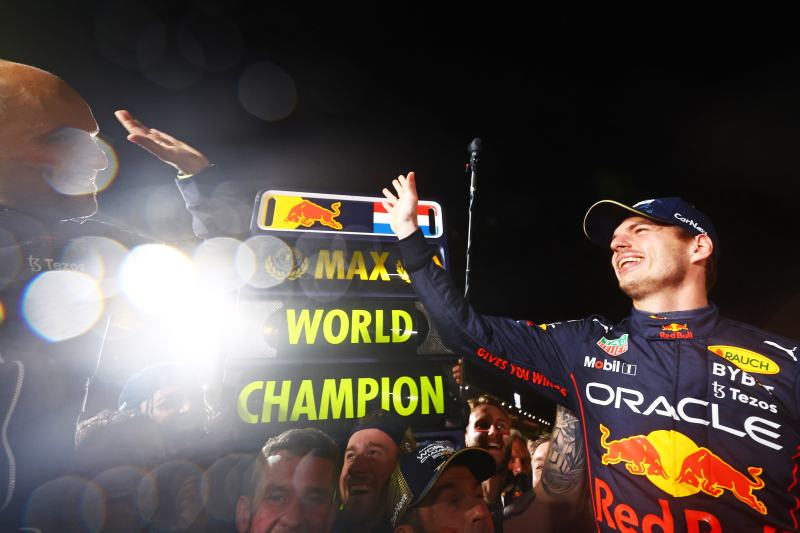
\includegraphics[scale = 2]{img/max}
            \caption{Max Verstappen - Mistrz Świata 2022}
            \label{fig:max}
        \end{figure}

    \newpage   
    \subsection{Najlepszy zespół}
        \begin{center}
            \Huge \textbf{Red Bull Racing}
        \end{center}
         Czerwone byki znów na tronie. Red Bull sięgnął po mistrzostwo konstruktorów, przerywając hegemonię Mercedesa. Przez praktycznie cały sezon, zespół Verstappena i Pereza nie miał godnego przeciwnika. Świetna maszyna i brak równej rywalizacji pozwolił zespołowi z Milton Keynes na jeden z najlepszych występów, jakie widział ten sport.\\

        Red Bull był praktycznie bezbłędny. Brak pomyłek strategicznych, szybcy kierowcy, krótkie pit stopy - przepis na sukces. Oprócz braku błędów, mistrzów trzeba pochwalić za niesamowitą umiejętność wykorzystywania słabości przeciwników oraz bardzo szybkiego dostosowywania się do rozmaitych sytuacji podczas wyścigów.\\
        
        RB18, dostarczony na tor przez Red Bulla, okazał się świetnym bolidem, mimo falstartu w początkowej fazie tegorocznej kampanii. Czerwone byki nie dojechały do mety GP Bahrajnu. Podczas ostatnich okrążeń, oba samochody napotkały problemy z układem paliwa. Problemy doprowadziły do przedwczesnego zakończenia rywalizacji. Szczęśliwym dla Verstappena nie był też wyścig w Melbourne, w którym również nie ujrzał flagi w szachownicę. Na szczęście kierowcy auta nr 1, reszta sezonu przebiegła bez żadnych awarii. Sergio Perez, oprócz Bahrajnu, tylko raz wycofywał się z powodu usterki (Kanada).\\
        
        Podsumowując występy zespołu, Red Bull uzbierał 17 zwycięstw, tylko cztery razy ustępując Ferrari, a raz - Mercedesowi. Do wybitnej statystyki wygranych, kierowcy stawali 28 razy na podium. Jednym słowem - klasa. 

        \begin{figure}[ht]
            \centering
            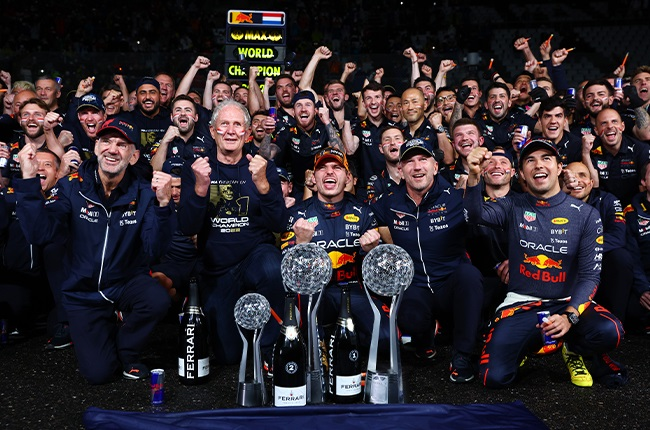
\includegraphics[scale = 2.3]{img/red-bull}
            \caption{Red Bull - Mistrz Świata 2022}
            \label{fig:rbr}
        \end{figure}
   
    \newpage 
    \subsection{Największe rozczarowanie (kierowca)}
        \begin{center}
            \Huge \textbf{Daniel Ricciardo}
        \end{center}

        Po drugim roku w McLarenie trzeba to powiedzieć wprost. Australijczyk w pomarańczowym aucie był słaby. Cień siebie z najlepszych lat kariery, kiedy jeździł w barwach Red Bulla. Rok zakończony beznadziejnie. W marcu na gridzie już go nie zobaczymy.\\

        Zaledwie 37 punktów zdobytych. W porównaniu ze 122 oczkami Lando Norrisa. Przepaść, ewidentna różnica. Ricciardo nigdy nie dostosował się do auta z Woking. Ciężko znaleźć coś na jego obronę - w zeszłym sezonie było o wiele lepiej. Była wygrana i było też 115 punktów.\\
        
        Ricciardo tylko dwa razy wygrał w kwalifikacjach z zespołowym kolegą. Przegrał aż 20. Pięć razy odpadał też w Q1, Norris zaś zawsze wchodził co najmniej do drugiej rundy. Słabej dyspozycji nie da się usprawiedliwić generalnymi problemami z samochodem. Pomijając początek sezonu i trudności z chłodzeniem hamulców, MCL36 sprawował się dobrze.\\
        
        Przykro się patrzy na niemoc sympatycznego Australijczyka. W 2023 roku będzie pełnił funkcję kierowcy rezerwowego w Red Bullu, a jego miejsce zajmuje Oscar Piastri.\\

        \begin{figure}[ht]
            \centering
            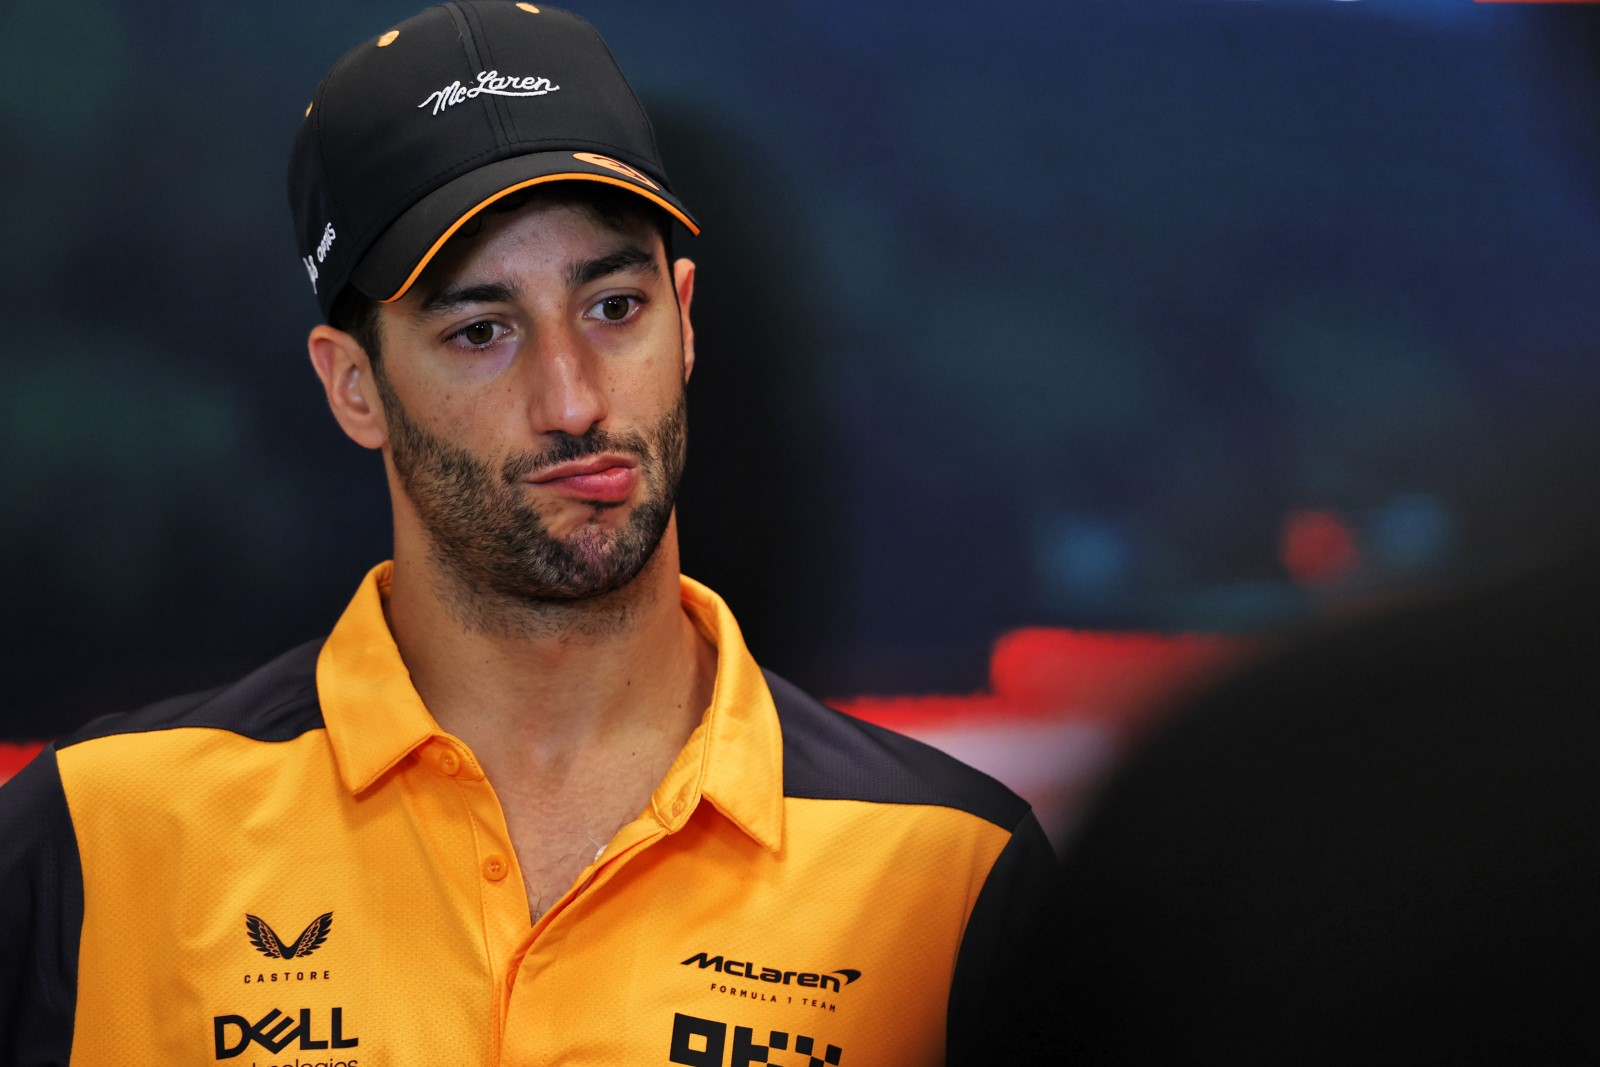
\includegraphics[scale = 1]{img/daniel-ricciardo}
            \caption{Daniel Ricciardo - McLaren}
            \label{fig:ricc}
        \end{figure}
        
    \newpage   
    \subsection{Największe rozczarowanie (zespół)}
        \begin{center}
            \Huge \textbf{Alpha Tauri}
        \end{center}

        Sezon iście przejściowy. Nowa konstrukcja aut, ale kierowcy i zespół ci sami. Rok słaby, bez przebłysków czegoś dobrego, mocnego. Trudności nie udało się przezwyciężyć. Sam spodziewałem się, że włoski zespół będzie jednym z tych lepszych. Tak bolesny upadek wydawał się być nierealny.\\

        Tegoroczny sezon zakończony praktycznie na dnie - niżej był tylko Williams. 35 punktów brzmi śmiesznie. A przecież w zeszłym roku było ich 142 i P6 w klasyfikacji konstruktorów. Teraz pozycja za Haasem. Aż ciężko w to uwierzyć. Ktoś musiał paść ofiarą nowych regulacji dotyczących konstrukcji bolidów - tym zespołem jest Alpha Tauri.\\
        
        Od następnego sezonu, miejsce Pierre’a Gasly’ego zajmie Nyck de Vries. Holender zadebiutował w wyścigu F1, w którym zdobył punkty w aucie Williamsa. Może będzie to dla włoskiego zespołu dobra zmiana, impuls, który pozwoli im walczyć o wyższe miejsce. 

        \begin{figure}[ht]
            \centering
            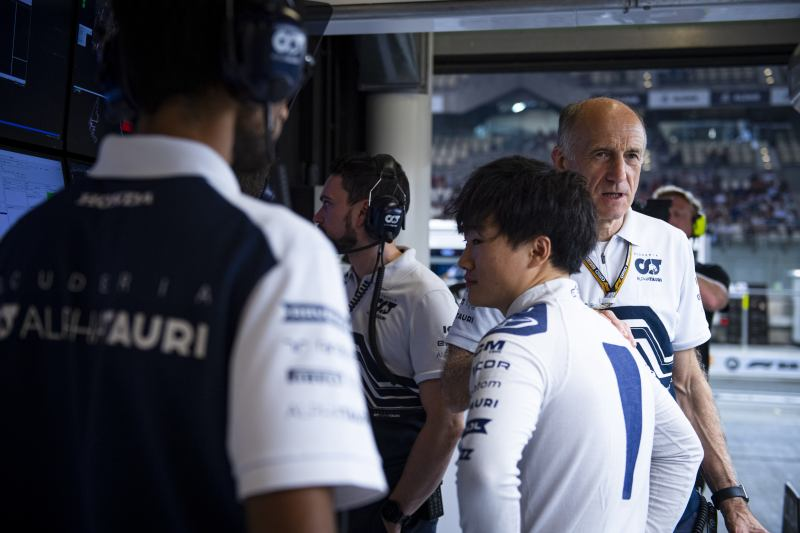
\includegraphics[scale = 2]{img/alpha-tauri}
            \caption{Szef zespołu Franz Tost oraz kierowca Yuki Tsunoda - Alpha Tauri}
            \label{fig:alpha}
        \end{figure}

    \newpage
    \subsection{Największe pozytywne zaskoczenie}
        \begin{center}
            \Huge \textbf{George Russell}
        \end{center}

        George Russell zaliczył próbę czasu w Williamsie. Owoce trudów początku jego kariery wreszcie kwitną. Miejsce w Mercedesie nie należało się bardziej nikomu innemu. Dobrze wiedział, że nie ma miejsca na błędy i słabości. Już w tym roku pokonał Lewisa Hamiltona w tym samym samochodzie.\\
        
        Brytyjczyk długo czekał na swoją kolej. Debiutując w Williamsie, czekał 37 wyścigów na pierwsze punkty. Zdobył je w barwach Mercedesa podczas GP Sakhir w 2020 roku, zastępując chorego na Covid Hamiltona. Od tamtego czasu było już pewne - Russell jest piekielnie szybki.\\
        
        Kiedy już dostał miejsce w zespole Toto Wolffa, zaczął z wysokiego C. Regularnie klasyfikował się wyżej od kolegi z zespołu. Dał też Mercedesowi jedyne, jakże upragnione zwycięstwo w Brazylii.\\
        
        George Russell był lepszy od Hamiltona w najważniejszych aspektach, między innymi lepiej prezentował się w wyścigach. Młodszy z Brytyjczyków w soboty zazwyczaj nie kwalifikował się wyżej od siedmiokrotnego mistrza. Jednak gdy go wtedy pokonywał, to z przytupem. Zdobył pole na Hungaroringu, wygrał sprint w Sao Paulo. Sezon zakończył z 275 punktami, pokonując zespołowego rywala o 35 punktów. Wschodząca gwiazda - Toto nie musi się martwić o kierowcę, który przejmie schedę po Lewisie Hamiltonie. 

        \begin{figure}[ht]
            \centering
            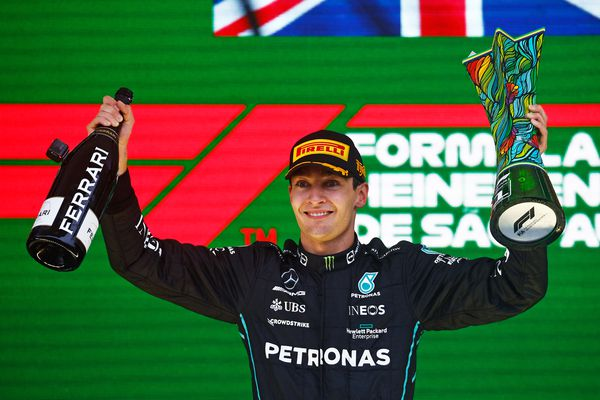
\includegraphics[scale = .6]{img/george-russell}
            \caption{George Russell - zwycięstwo w Brazylii}
            \label{fig:russell}
        \end{figure}
        
    \newpage  
    \subsection{Najlepszy debiut/powrót}
        \begin{center}
            \Huge \textbf{Kevin Magnussen}
        \end{center}

        Powrót przyszedł nagle. Jednak Guenther Steiner i Gene Haas musieli szybko kogoś znaleźć za Mazepina, który jako Rosjanin został zawieszony - padło na Duńczyka. Chyba nikt nie spodziewał się, że Magnussen, który rok wcześniej żegnał się z amerykańskim zespołem, będzie głównym kreatorem zaskakującej dyspozycji Haasa.\\

        K-Mag świetnie się zaprezentował. Zdobył 25 punktów, co z 12 punktami Schumachera, dało Haasowi ósme miejsce w klasyfikacji. Coś niebywałego - po poprzednim sezonie, gdzie nie zdobyli żadnego punktu, teraz kończą z dorobkiem 37 oczek.\\
        
        Magnussen nie mógł lepiej wymarzyć sobie pierwszego wyścigu po powrocie. P5 w Grand Prix Bahrajnu; Steiner po fladze w szachownicę powiedział mu przez radio, że powrócił do Formuły 1 niczym wiking. I ma w pełni rację.\\
        
        Magiczny sezon dopełnia zdobyte pole position podczas weekendu w Sao Paulo. Wiadomo, dużą rolę odegrało tam szczęście i zmienna pogoda, jednak kto będzie to pamiętać. Ważne, że Kevin został reprezentantem 24. kraju, który zajął pierwszą pozycję po kwalifikacjach.\\

        \begin{figure}[ht]
            \centering
            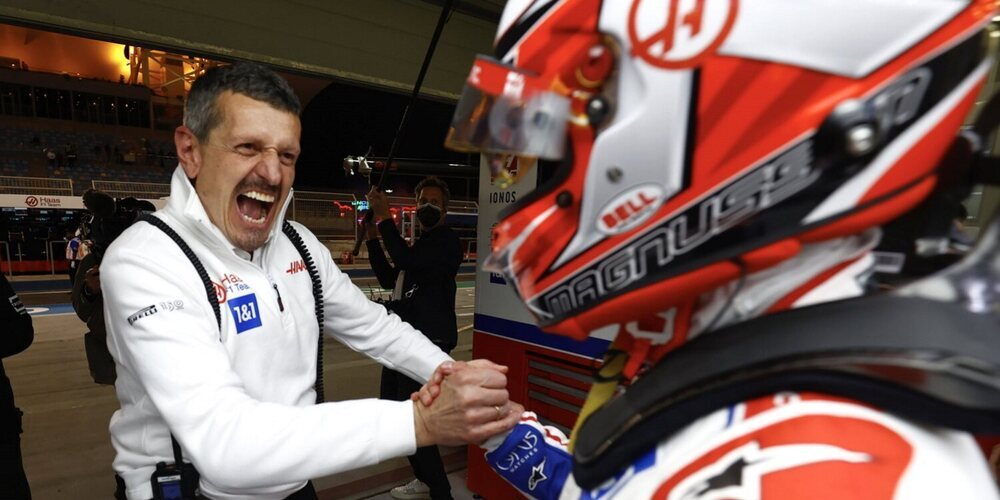
\includegraphics[scale = .55]{img/kevin-magnussen}
            \caption{Kevin Magnussen - zwycięzca deszczowych kwalifikacji w Brazylii}
            \label{fig:magnussen}
        \end{figure}

    \newpage
    \subsection{Najlepszy wyścig}
        \begin{center}
            \Huge \textbf{Grand Prix Wielkiej Brytanii}
        \end{center}

        Na torze w Silverstone zawsze można spodziewać się dobrej rywalizacji. Nie inaczej było w tym roku - fantastyczny, ale również dramatyczny wyścig, trzymający w emocjach od początku do końca.\\

        Sobotnie kwalifikacje konkludowały pierwszym pole position dla Carlosa Sainza. Wyścig nie był dla Hiszpana spacerkiem. Po wymagającej niedzieli, Hiszpan również sięgnął po swoje pierwsze zwycięstwo w królowej motorsportu.\\
        
        Rozpoczęło się od chaosu i groźnych wypadków Zhou, Albona i Russella. Chińczyk po kolizji z Brytyjczykiem dachował i praktycznie wypadł poza tor. Ściganie natychmiast przerwano. Po wznowieniu zostaliśmy uraczeni jedną z najlepszych walk w tym sezonie, w której udział brali kierowcy Ferrari oraz Red Bulla. Rywalizacja między nimi trwała parę okrążeń, aż do momentu, gdy problemy z samochodem zaczął mieć Verstappen.\\
        
        W końcówce namieszał Esteban Ocon, który z powodu awarii musiał zatrzymać się na torze. Nastąpiła neutralizacja; po niej zostało zaledwie dziesięć okrążeń pod zieloną flagą. W pogoń za Sainzem rzucił się Perez, jednak między nimi nadal znajdował się Leclerc. Podczas próby wyprzedzenia Monakijczyka, z okazji szerokiego wyjazdu w ostatnim zakręcie kierowców Red Bulla i Ferrari skorzystał Lewis Hamilton, dokonując jednego z najładniejszych manewrów tego sezonu. 

        \begin{figure}[ht]
            \centering
            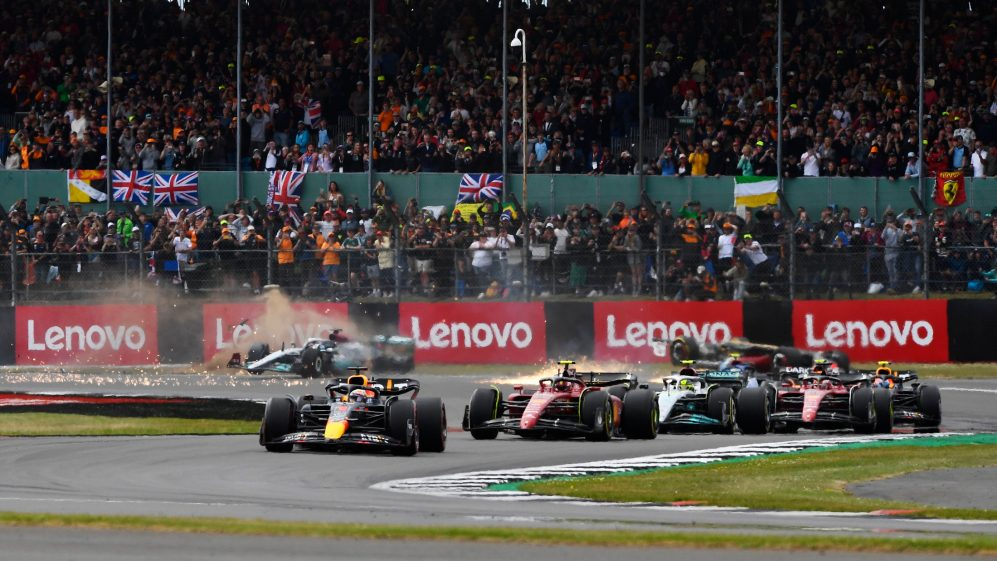
\includegraphics[scale = .4]{img/silverstone}
            \caption{Pędząca czołówka, a w tle kolizja Russella i Zhou - Silverstone}
            \label{fig:silverstone}
        \end{figure}

    \newpage
    \subsection{Najgorszy wyścig}
        \begin{center}
            \Huge \textbf{Grand Prix Japonii}
        \end{center}

        Formuła 1 ostatni raz gościła w Kraju Kwitnącej Wiśni podczas sezonu 2019. Wtedy Mercedes zapewnił sobie szósty mistrzowski tytuł. Mimo to, rywalizacja sprzed trzech lat nie zapadła szczególnie w pamięć. Ostatni wyścig, podobnie jak ten poprzedni, nie zapisze się złotymi zgłoskami w historii motorsportu.\\

        Warunki na torze były dramatyczne - ogromna ulewa. Na pierwszym okrążeniu, ściganie się już zakończyło. Na tor wyjechał samochód bezpieczeństwa, a na trzecim okrążeniu wywieszono czerwoną flagę.\\
        
        Sesja była zatrzymana przez ponad dwie godziny. Razem ze startem wyścigu, odliczanie rozpoczął zegar trzech godzin, po zakończeniu którego następuje wywieszenie flagi z szachownicą. Pozostawiło to kierowcom i kibicom niecałe 50 minut ścigania, poprzedzone bardzo długim oczekiwaniem.\\
        
        Wyścig nie zachwycił; gdyby nie zdobycie tam mistrzostwa przez Verstappena, puścilibyśmy weekend w Japonii w niepamięć. Tegoroczna wizyta w Suzuce pokazała, że potrzeba zmian w rozgrywaniu deszczowych sesji jest duża.\\

        \begin{figure}[ht]
            \centering
            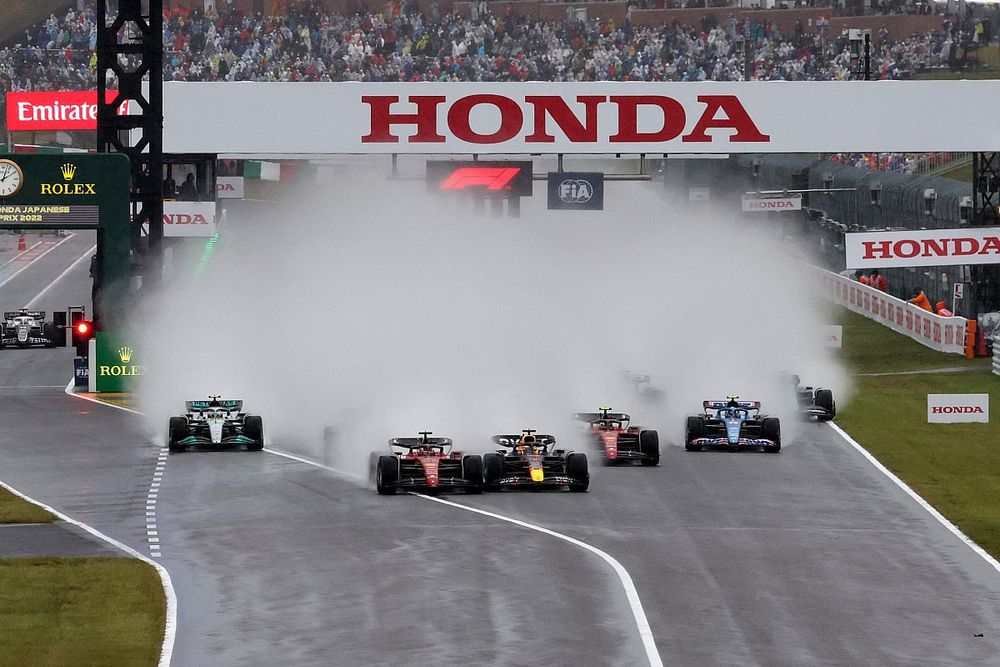
\includegraphics[scale = .4]{img/suzuka.jpg}
            \caption{Start deszczowego Grand Prix - Suzuka}
            \label{fig:japan}
        \end{figure}
        
\end{document}
